\documentclass{article}

\usepackage{graphicx}
\usepackage{tikz}
\usepackage{tikzsymbols}
\usetikzlibrary{calc,patterns,shapes.geometric}
\pagestyle{empty}
\usepackage[margin=0pt]{geometry}
\geometry{papersize={14in,12in}}

\def\centerarc[#1](#2)(#3:#4:#5){\draw[#1] ($(#2)+({#5*cos(#3)},{#5*sin(#3)})$) arc (#3:#4:#5);}

\begin{document}
	\begin{figure}
		\centering
		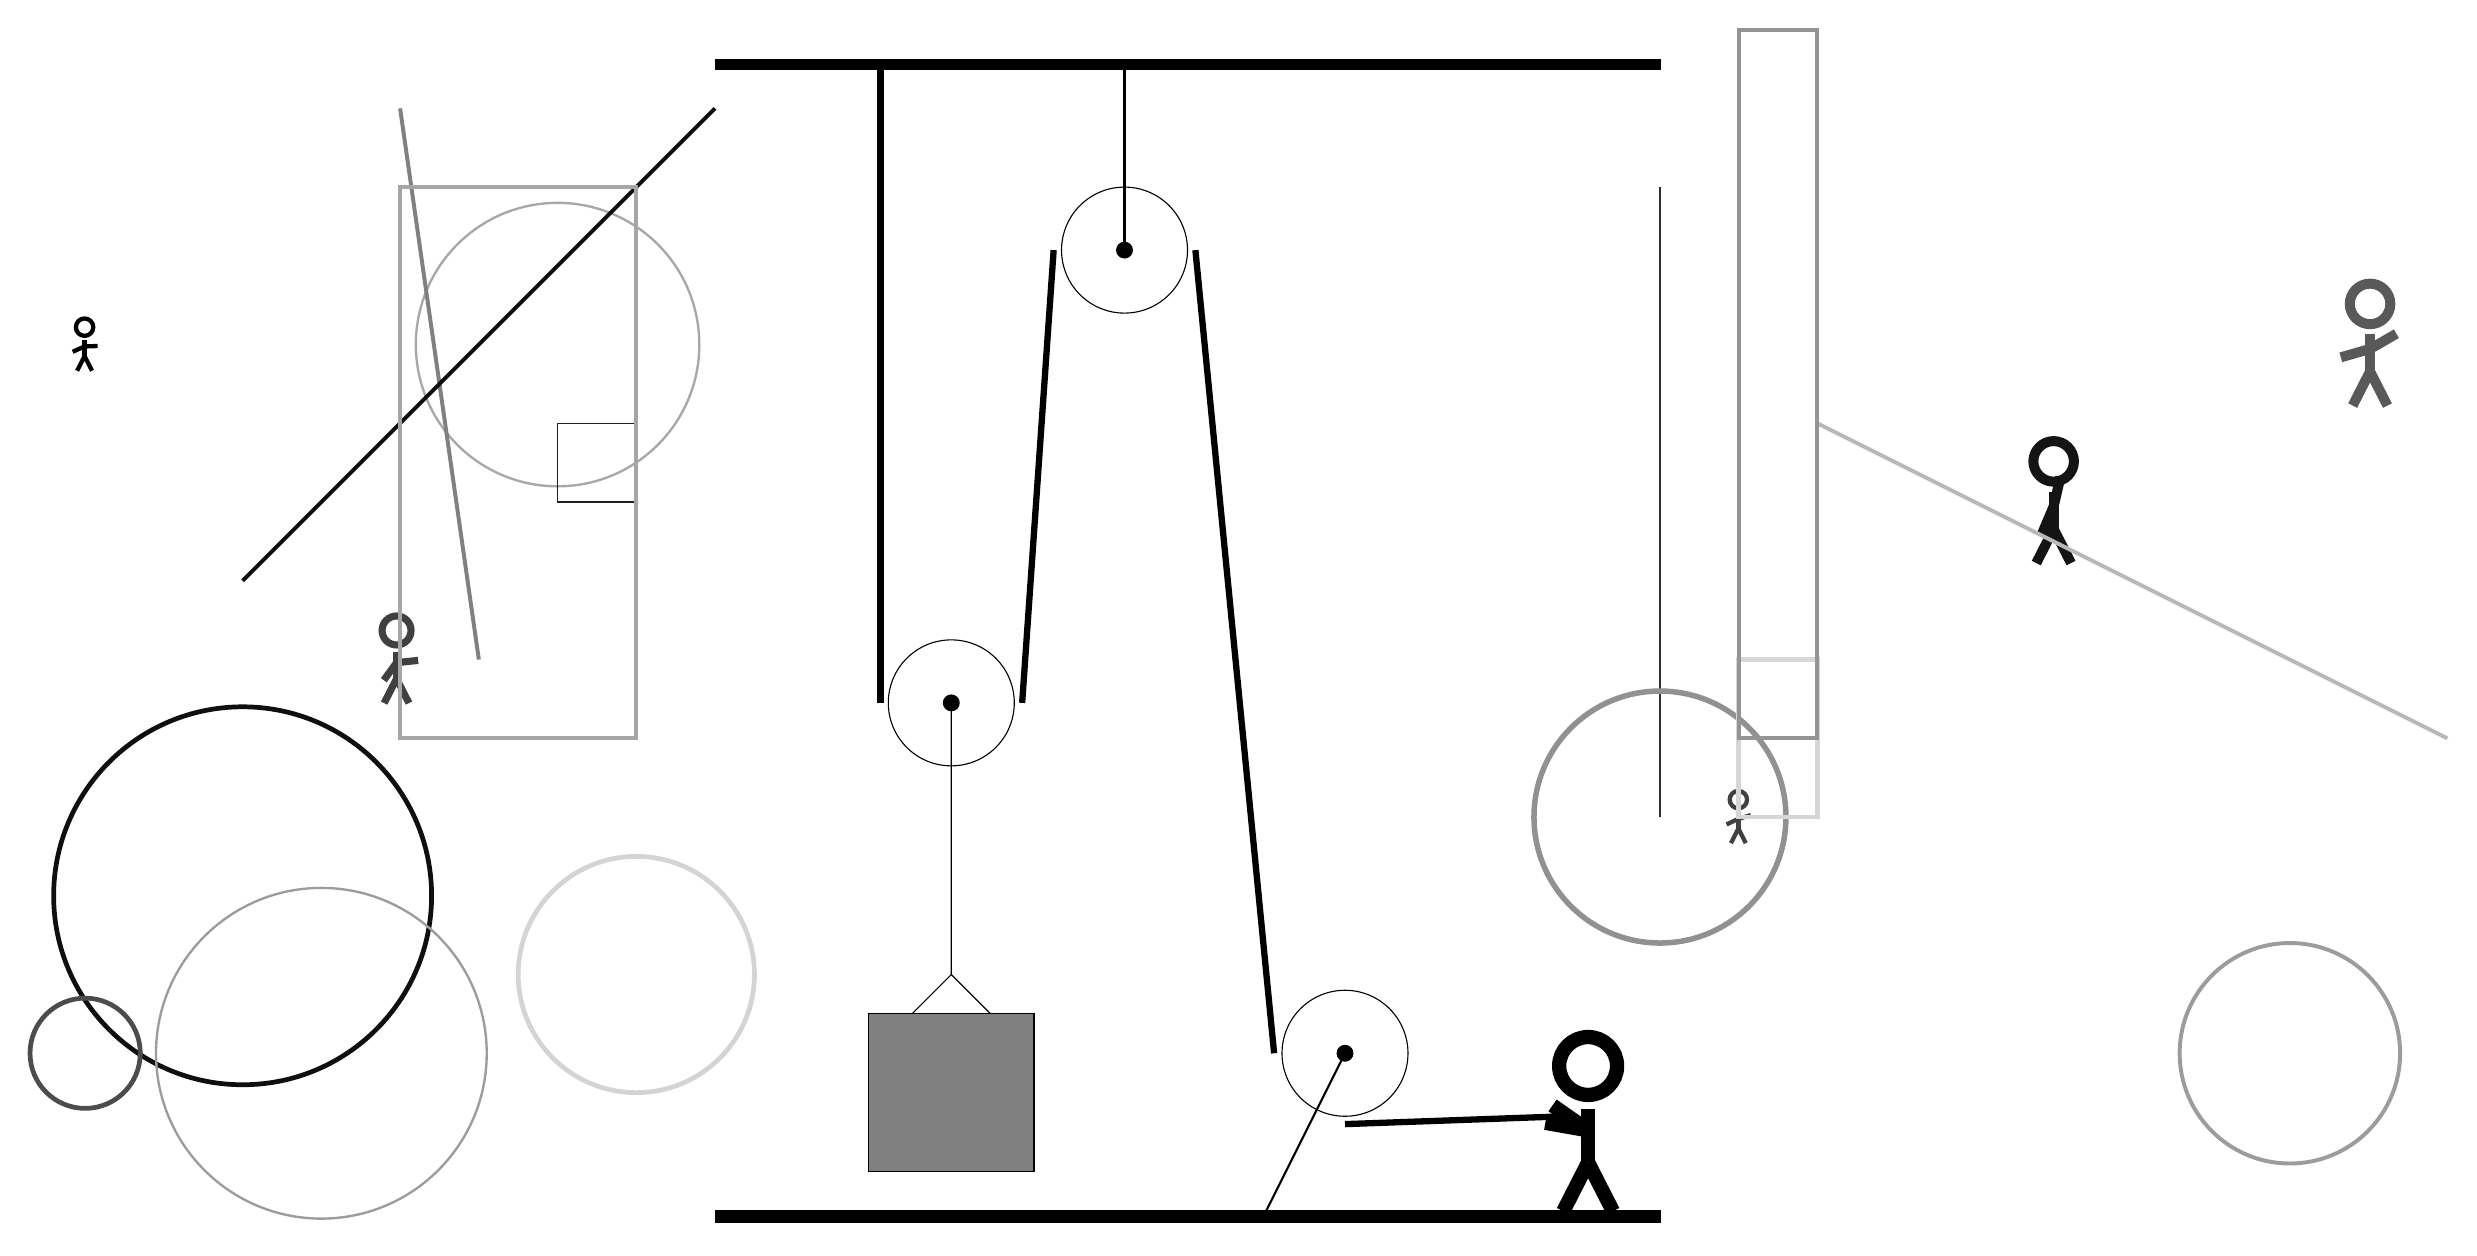
\begin{tikzpicture}
			%%%%% START %%%%%
			
			\draw[fill=black] (-2, 11.5) rectangle (10, 11.625);
			
			\draw (3.2, 9.2) circle (0.8);
			\draw[fill=black] (3.2, 9.2) circle (0.1);
			\draw[thick] (3.2, 9.2) -- (3.2, 11.5);
			
			\draw [line width=0.6mm, color=black!94](-8, 1) circle (2.4);
			
			\node[line width=0.3mm, color=black!65] at (19, 8) {\Strichmaxerl[7][16][30]};
			\draw[line width=0.5mm, color=black!49](-3, 4) -- (-3, 6);
			\draw [line width=0.6mm, color=black!70](-10, -1) circle (0.7);
			\draw [line width=0.6mm, color=black!17](-3, 0) circle (1.5);
			
			\draw[line width=0.2mm, color=black!82] (10, 10) rectangle (10, 2);
			\node[line width=0.4mm, color=black!100] at (-10, 8) {\Strichmaxerl[3][24][2]};
			
			\draw [line width=0.7mm, color=black!43](10, 2) circle (1.6);
			\draw [line width=0.3mm, color=black!39](-7, -1) circle (2.1);
			\draw [line width=0.3mm, color=black!34](-4, 8) circle (1.8);
			\node[line width=0.7mm, color=black!75] at (11, 2) {\Strichmaxerl[3][25][17]};
			\node[line width=0.5mm, color=black!92] at (15, 6) {\Strichmaxerl[7][67][77]};
			\draw[line width=0.5mm, color=black!28](12, 7) -- (20, 3);
			
			\draw[line width=0.6mm, color=black!16] (12, 2) rectangle (11, 4);
			\draw[line width=0.5mm, color=black!50](-6, 11) -- (-5, 4);
			\draw[line width=0.2mm, color=black!88] (-3, 6) rectangle (-4, 7);
			
			\draw [line width=0.5mm, color=black!39](18, -1) circle (1.4);
			
			\node[line width=0.4mm, color=black!75] at (-6, 4) {\Strichmaxerl[5][54][6]};
			\draw[line width=0.5mm, color=black!94](-2, 11) -- (-8, 5);
			
			\draw[line width=0.5mm, color=black!42] (12, 3) rectangle (11, 12);
			\draw[line width=0.5mm, color=black!35] (-3, 3) rectangle (-6, 10);
			
			\draw (6, -1) circle (0.8);
			\draw[fill=black] (6, -1) circle (0.1);
			\draw[thick] (6, -1) -- (5, -3);
			
			\draw (1, 3.45) circle (0.8);
			\draw[fill=black] (1, 3.45) circle (0.1);
			
			\draw (1, 3.45) -- (1, 0.0) -- (0.5, -0.5);
			\draw (1, 0.0) -- (1.5, -0.5);
			\draw[fill=black!50] (-0.05, -0.5) rectangle (2.05, -2.5);
			
			\draw[line width=0.8mm] (0.1, 11.5) -- (0.1, 3.45);
			\centerarc[line width=0.8mm](1, 3.45)(180:360:0.9);
			\draw[line width=0.8mm](1.9, 3.45) -- (2.3, 9.2);
			\centerarc[line width=0.8mm](3.2, 9.2)(0:180:0.9);
			\draw[line width=0.8mm](4.1, 9.2) -- (5.1, -1);
			\centerarc[line width=0.8mm](6, -1)(180:270:0.9);
			\draw[line width=0.8mm](6, -1.9) -- (8.8, -1.8);
			
			\node at (9, -1.9) {\Strichmaxerl[10][-35][170]};
			
			\draw[fill=black] (-2, -3) rectangle (10, -3.15);
			
			%%%%% END %%%%%
		\end{tikzpicture}
	\end{figure}	
\end{document}